\documentclass[a4paper, 11pt]{llncs}
\usepackage{url}
\usepackage{graphicx}
\usepackage{comment}
\usepackage{printlen} % Print lengths using specified units. 
%\usepackage{hyperref}
\usepackage{booktabs}
\usepackage[utf8]{inputenc} % Umlaute üöä auch normal benutzen und nicht maskieren
\usepackage[rightcaption]{sidecap}  % caption beside figure
\usepackage{color}

% http://www.ctan.org/tex-archive/fonts/ps-type1/cm-super/
\usepackage[T1]{fontenc} % use high quality fonts, please install cm-super


%%%% LISTINGS
\usepackage{listings} % Typeset source code listings using LaTeX.
% listing styles
\lstset{%
    numberbychapter=false,
    numbers=left,
    numberstyle=\tiny,
    basicstyle=\ttfamily\small,
    tabsize=2,
    framexleftmargin=2pt,
    captionpos=b,
    frame=single,
    breaklines=true
}
%\lstdefinestyle{rdf}{numberblanklines=true, morekeywords={}}
%\lstdefinestyle{sparql}{numberblanklines=true, morekeywords={SELECT,WHERE FILTER, GROUP BY, IN, AS}}
\lstdefinestyle{N3}{numberblanklines=true, morekeywords={foaf, prefix}}

%%%% todo
%\newcommand{\todo}[1]{\emph{\textbf{[ToDo: #1]}}}
% draws PDF notes instead of in-text todos
%\usepackage{pdfmarginpar}\newcommand{\todo}[1]{\pdfmarginpar[Note]{ToDo: #1}}
\newcommand{\todo}[1]{}


\newcommand{\NAME}{Creating Knowledge out of Interlinked Data: The Integrated LOD2 Tool Stack}

\pdfinfo {%
	/Title (\NAME)
	/Creator (TeX)
	/Producer (pdfTeX and Document $Revision$)
	/Author (Sebastian Tramp, Bert Van Nuffelen, Michael Martin and Soeren Auer)
	%/CreationDate (D:19980212201000)
	%/ModDate (D:19980212201000)
	/Subject (\NAME)
}

\graphicspath{{images/}} % include-pfad für Grafiken
\DeclareGraphicsExtensions{.pdf,.png}

\begin{document}

\title{\NAME}

\titlerunning{\NAME}

\author{Bert Van Nuffelen \and Sebastian Tramp \and Sören Auer}

\authorrunning{Sebastian Tramp et al.}

\institute{%
Universit\"at Leipzig, Institut f\"ur Informatik, AKSW,\\
Postfach 100920, D-04009 Leipzig, Germany,\\
\email{\{lastname\}@informatik.uni-leipzig.de}\\
\url{http://aksw.org}
}

\maketitle              % typeset the title of the contribution

\begin{abstract}
This joint tutorial of the consortium of the European IP project LOD2 - Creating Knowledge out of Interlinked Data will give an overview on the area of creating, managing and using Linked Data sources.
As a prerequisite to the main tutorial part, we give an overview of the life cycle of Linked Data usage and its challenges as well as the LOD2 software stack, which is an integrated distribution of aligned tools which support the life-cycle of Linked Data from extraction, authoring/creation over enrichment, interlinking, fusing to visualization and maintenance. 
Based on this more theoretic explanations, we give a detailed insight into the usage of LOD2 stack both with practical and non-practical parts.
More specifically, we present tools and usage scenarios for the following Linked Data life cycle tasks: extraction (Triplify / D2R), storage and querying (Openlink Virtuoso), authoring and manual revision (OntoWiki), interlinking and fusion (Silk / LIMES) and enrichment and repair (ORE).
In addition to that, we present the LOD2 stack demonstrator which integrates these and other LOD2 tools for a better user experience.
\end{abstract}

\section{Introduction}

LOD2 is a large-scale integrating project co-funded by the European Commission within the FP7 Information and Communication Technologies Work Programme (Grant Agreement No. 257943).
Commencing in September 2010, this 4-year project comprises leading Linked Open Data technology researchers, companies, and service providers (15 partners) from across 11 European countries (and one associated partner from Korea) and is coordinated by the AKSW research group at the University of Leipzig.

The goals of the LOD2 project include the development of enterprise-ready tools and methodologies for exposing and managing very large amounts of structured information on the Data Web and adaptive tools for searching, browsing, and authoring of Linked Data.
These tools are distributed as the LOD2 stack.
The LOD2 stack is an integrated distribution of aligned tools which support the life-cycle of Linked Data (depicted in Figure~\ref{fig:lifecycle}) from extraction, authoring/creation over enrichment, interlinking, fusing to visualization and maintenance.

\begin{figure}[t]
	\centering
		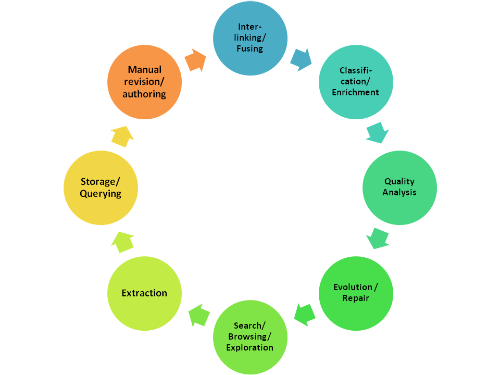
\includegraphics[width=0.95\textwidth]{lod-lifecycle-small}
	\caption{Linked Data Lifecycle}
	\label{fig:lifecycle}
\end{figure}

\section{The Tutorial}

%Tutorial proposals should not exceed 5 pages, using an 11 pt font for
%the body of the text of the proposal and should contain the following
%information: Abstract (200 words maximum, for inclusion on the ESWC 2012
%website).
    
%Tutorial description: More specifically, it should

The tutorial will give an overview to the complete LOD2 stack and a detailed insight to the integrated tools in Sec.\ref{sec:stack}.
For each tool we will give a talk followed by a practical part.
Each practical part is guided by an overall usage scenario which covers most parts of the Linked Data life cycle.
For the practical parts, we provide a virtual machine where the LOD2 stack and additional material is already installed (slides, data sources, software packages).

The intended audience covers knowledge workers from the industry which need to integrate and use Linked Data from different open and non-open data sources as well as researchers and PhD students which are new in the area of Linked Data.

This is a full day tutorial and it was never given before on other venues.

% * specify the objective of the tutorial and relevance to ESWC 2012
% * include enough details on the scope of the material to be covered and
%   the depth to which it will be covered and
% * specify the intended audience and any prerequisite knowledge.
%   Appropriate references to the material to be covered by the tutorial
%    must be included.

%Tutorial length. The tutorial can be full or half day (if the tutorial
%can be either length, please be sure to identify which material is
%included for each length).
    
%Other venues to which the tutorial or part thereof has or will be
%presented, and explain how the current tutorial differs from the other
%editions. Links to the slides of those tutorial editions should be
%included in the proposal.

\section{The Presenters}

%Brief professional biography of the presenter(s) indicating previous
%training and speaking experience (such as teaching and tutorial
%presentation).

Dr. S\"oren Auer 

Dr. Bert Van Nuffelen 

Sebastian Tramp studied information science and is a research associate at AKSW / University of Leipzig since 2006.
He is author of over 30 peer-reviewed publications and presented his research projects on conferences as the ESWC and the ISWC as well as multiple workshops
He is a lecturer at the University of Leipzig and the Leipzig School of Media.

    
\section{The LOD2 Stack}
\label{sec:stack}

The LOD2 stack comprises new and substantially extended existing tools from the LOD2 partners and third parties.
The LOD2 stack is organized as a Debian package repository making the tool stack easy to install on any Debian-based system (e.g. Ubuntu).
In our tutorial, we present tools and usage scenarios for the following Linked Data life cycle tasks:

\subsection{Extraction}

Triplify \cite{triplify_www} provides a building block for the "semantification" of Web applications.
Triplify is a small plugin for Web applications, which reveals the semantic structures encoded in relational databases by making database content available as RDF, JSON or Linked Data.
%Triplify is very lightweight: It consists of only a few files with less than 500 lines of code.
%For a typical Web application a configuration for Triplify can be created in less than one hour and if this Web application is deployed multiple times (as most open-source Web applications are), the configuration can be reused without modifications.
%Triplify makes Web applications easier mashable and lays the foundation for next-generation, semantics-based Web searches.

The D2R Server \cite{d2rposter} is a tool for publishing the content of relational databases on the Semantic Web.
D2R Server uses a customizable D2RQ mapping to map database content into RDF triple, and allows the RDF knowledge bases to be browsed and searched - the two main access paradigms to the Semantic Web.

\subsection{Storage and Querying}

Virtuoso \cite{virtuoso} is an innovative industry standards compliant platform for native data, information, and knowledge management.
It implements and supports a broad spectrum of query languages, data access interfaces, protocols, and data representation formats that includes SPARQL, RDF, RDFa and many more.
The open-source edition of Virtuoso, which includes a scalable high-performance RDF Quad Store, is be the basis for the LOD2 Stack's knowledge store.

\subsection{Authoring and Manual Revision}

OntoWiki \cite{auer-s-2006-736-a} is a tool providing support for agile, distributed knowledge engineering scenarios.
It facilitates the visual presentation of a knowledge base as an information map, with different views on instance data.
It enables intuitive authoring of semantic content, with an inline editing mode for editing RDF content, similar to WYSIWIG for text documents.
OntoWiki provides sophisticated means for navigating, visualising and authoring of RDF-based Knowledge Bases.
It serves and consumes Linked Data and comprises a comprehensive middleware API for building custom Semantic Web applications.

\subsection{Interlinking and Fusion}

The Silk Link Discovery Framework \cite{silk} supports data publishers in interlinking RDF knowledge bases.
Using the declarative Silk - Link Specification Language (Silk-LSL), developers can specify which types of RDF links should be discovered between data sources as well as which conditions data items must fulfill in order to be interlinked.
These link conditions may combine various similarity metrics and can take the graph around a data item into account, which is addressed using an RDF path language.

LIMES \cite{limes} is a link discovery framework for the Web of Data.
It implements time-efficient approaches for large-scale link discovery based on the characteristics of metric spaces.
It is easily configurable via a web interface. It can also be downloaded as standalone tool for carrying out link discovery locally.

\subsection{Enrichment and Repair}

ORE \cite{lehmann-2010-iswc} is a tool for repairing and enriching OWL ontologies.
State-of-the-art methods in ontology debugging and supervised machine learning form
the basis of ORE and are adapted or extended so as to work well in practice.
ORE supports the detection of a variety of ontology modelling problems and guides
the user through the process of resolving them.
Furthermore, the tool allows to extend an ontology through (semi-)automatic supervised learning.
A wizard-like process helps the user to resolve potential issues after axioms are added.




\paragraph*{Acknowledgments}
%We would like to thank our colleagues from AKSW research group for their helpful comments and inspiring discussions during the development of this approach.
This work was supported by a grant from the European Union's 7th Framework Programme provided for the project LOD2 (GA no. 257943).

\enlargethispage{2mm}

\bibliographystyle{plain}
\bibliography{tutorial}

\end{document}

